\documentclass[aspectratio=169,17pt]{beamer}
\usepackage{newtxtext,newtxmath}
\usepackage[utf8]{inputenc}
\usepackage[spanish]{babel}
\usepackage{graphicx}
\usepackage[backend=bibtex,style=numeric]{biblatex}
\addbibresource{Bibliografía.bib}
\usetheme{Madrid}

%           -------Infotrmación-------
\title[Fundamentos y Aplicación de la XR]
    {Fundamentos y Aplicación de la Realidad Extendida}
\author[Dr. Francisco Somarriba]
    {Dr. Francisco Somarriba López\inst{1}}
\institute[UCN]
    {
        \inst{1}
        Doctor en Medicina y Cirugía\\
        Facultad de Ciencias Médicas\\
        Universidad Central de Nicaragua
    }
\date[Mayo, 2025]

\begin{document}

%           -------Portada-------
\titlepage

%           -------Slides-------
    \begin{frame}{Contenido}
    \setbeamertemplate{section in toc}{
        \leavevmode\leftskip=2em\llap{\textbullet\hskip1em}\inserttocsection\par
    }
    \tableofcontents
    \end{frame}

\section{Introducción}
    \begin{frame}
        \frametitle{Introducción}
            La Realidad Extendida (XR), está transformando la forma en que interactuamos con el mundo digital. Su impacto se ha expandido más allá del entretenimiento, incursionando diversos ambitos.\\
            Esta presentación ofrece un recorrido por los fundamentos de la XR, su estado actual, usos personales de aplicación y una vista a las proyecciones futuras.
    \end{frame}

\section{Terminología esencial}
    \begin{frame}
        \frametitle{Terminología esencial}
            \textbf{Realidad virtual (VR):} inmersión en un entorno totalmente digital.\\
            \textbf{Realidad aumentada (AR):} superposición de una capa renderizada sobre el mundo real.\\
            \textbf{Realidad mixta (MR):} integración del mundo real y el renderizado. Crea una interacción directa entre el mundo digital y físico a la vez.
    \end{frame}
    
    \begin{frame}{Terminología esencial}
        \begin{figure}[ht]
            \begin{minipage}[b]{0.30\linewidth}
                \centering
                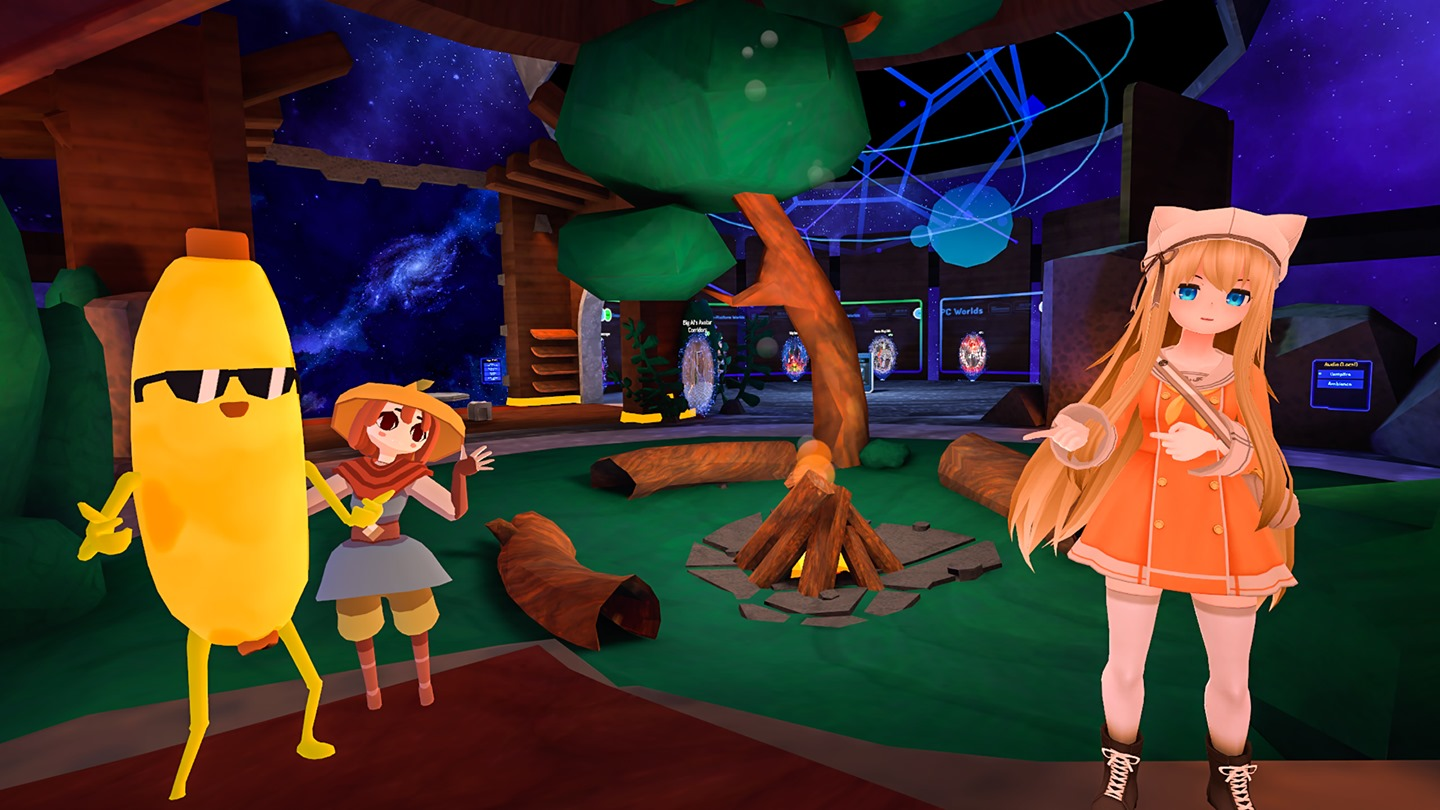
\includegraphics[width=\textwidth]{Ilustración 1.jpg}
                \caption{Entornos VR}
                \label{Ilu1}
            \end{minipage}
            \hspace{0.2cm}
            \begin{minipage}[b]{0.30\linewidth}
                \centering
                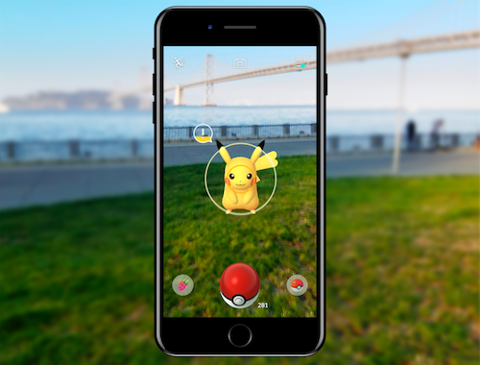
\includegraphics[width=\textwidth]{Ilustración 2.png}
                \caption{Entornos AR}
                \label{Ilu2}
            \end{minipage}
            \hspace{0.2cm}
            \begin{minipage}[b]{0.30\linewidth}
                \centering
                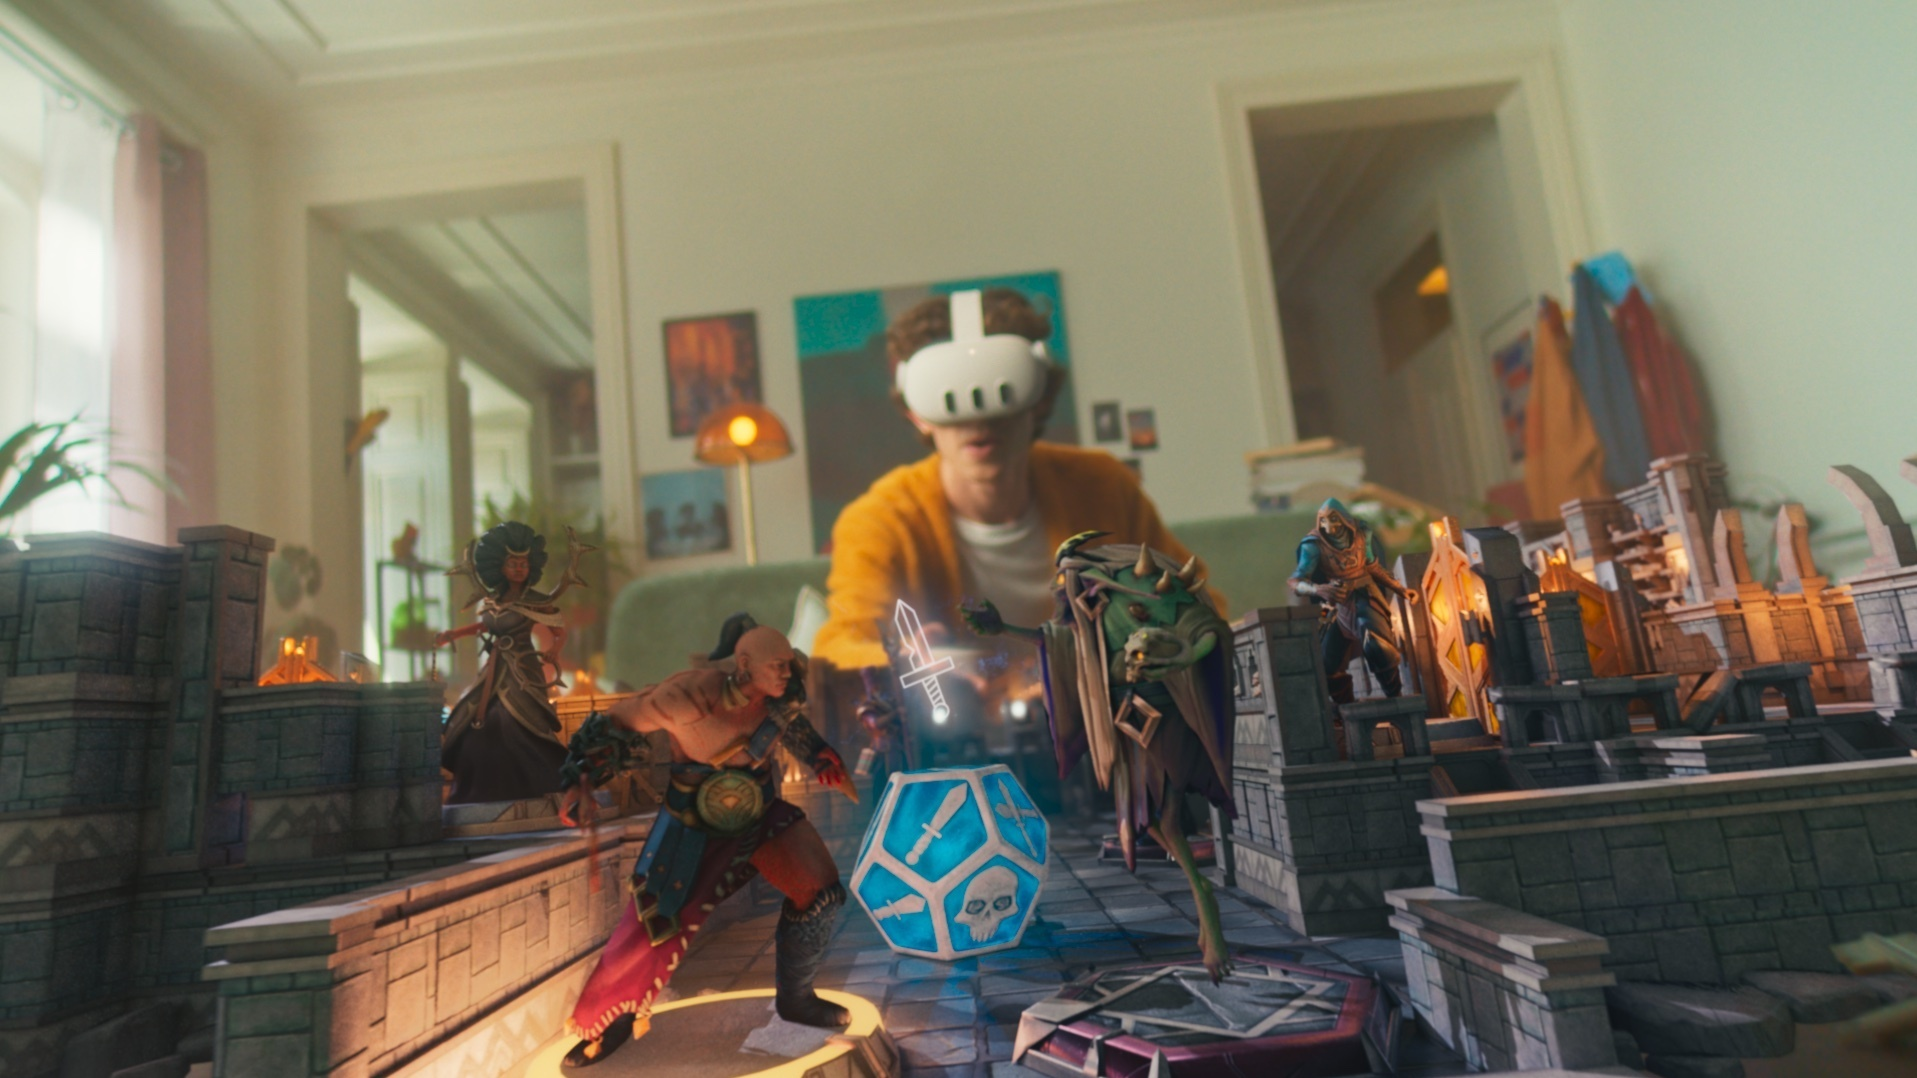
\includegraphics[width=\textwidth]{Ilustración 3.jpg}
                \caption{Entornos MR}
                \label{Ilu3}
            \end{minipage}
        \end{figure}
    \end{frame}
    
    \begin{frame}
        \frametitle{Terminología esencial}
            \textbf{Realidad extendida (XR):} término colectivo que se refiere a las tecnologías inmersivas, incluida VR, AR y MR.
    \end{frame}

    \begin{frame}
        \frametitle{Terminología esencial}
            \begin{figure}
                \centering
                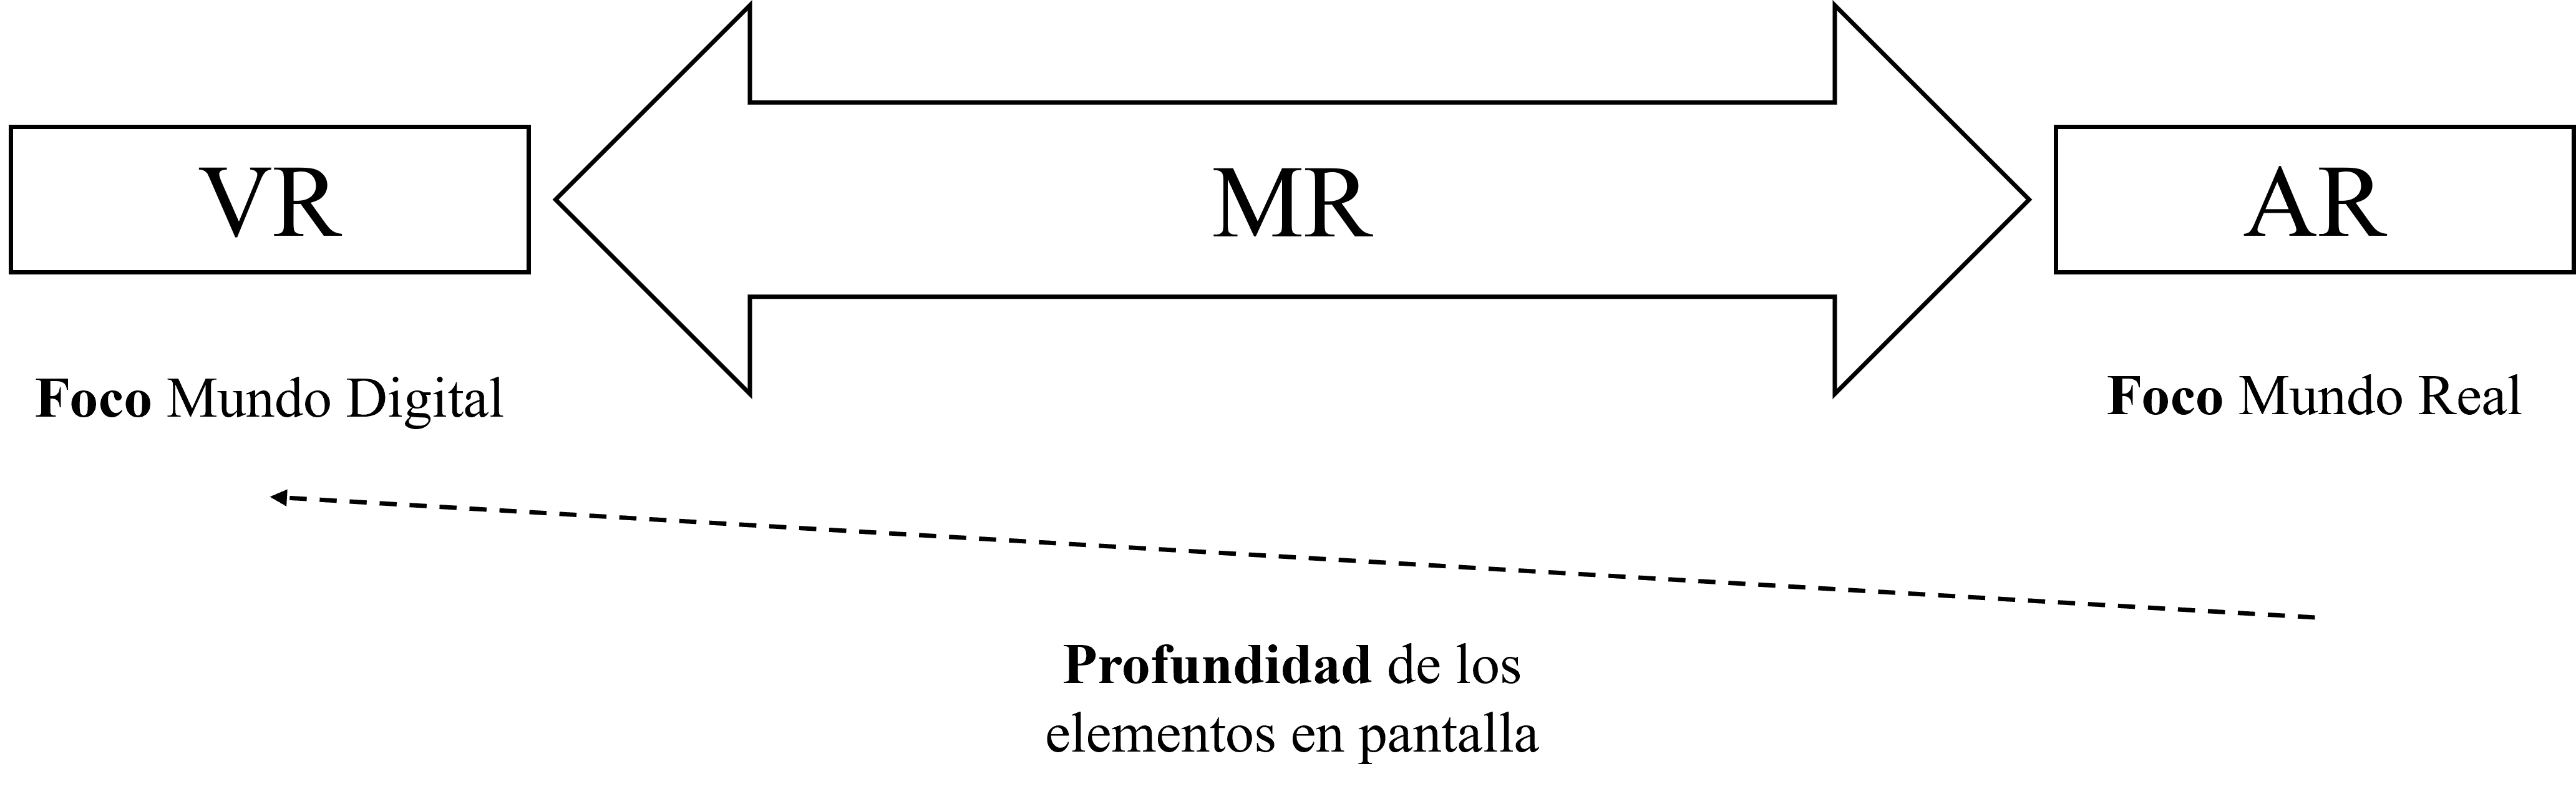
\includegraphics[width=1\linewidth]{Gráfica 1.png}
                \caption{Relación Foco/Profundidad en los entornos de XR}
                \label{Grá1}
            \end{figure}
    \end{frame}

    \begin{frame}
        \frametitle{Terminología esencial}
            \textbf{Tethered:} se conenctan a un dispositivo externo mediante cable para ocupar el hardware de este.\\
            \textbf{Standalone:} no requieren conectarse a un dispositivo externo, cuenta con su propio hardware.\\
            \textbf{Hybrid:} pueden funcionar como gafas tethered y standalone.\\
            \textbf{Smartphone:} funcionan como soporte para utilizar el hardware del teléfono. Simula ser un headset standalone.
    \end{frame}

    \begin{frame}
        \frametitle{Terminología esencial}
            \begin{figure}
                \centering
                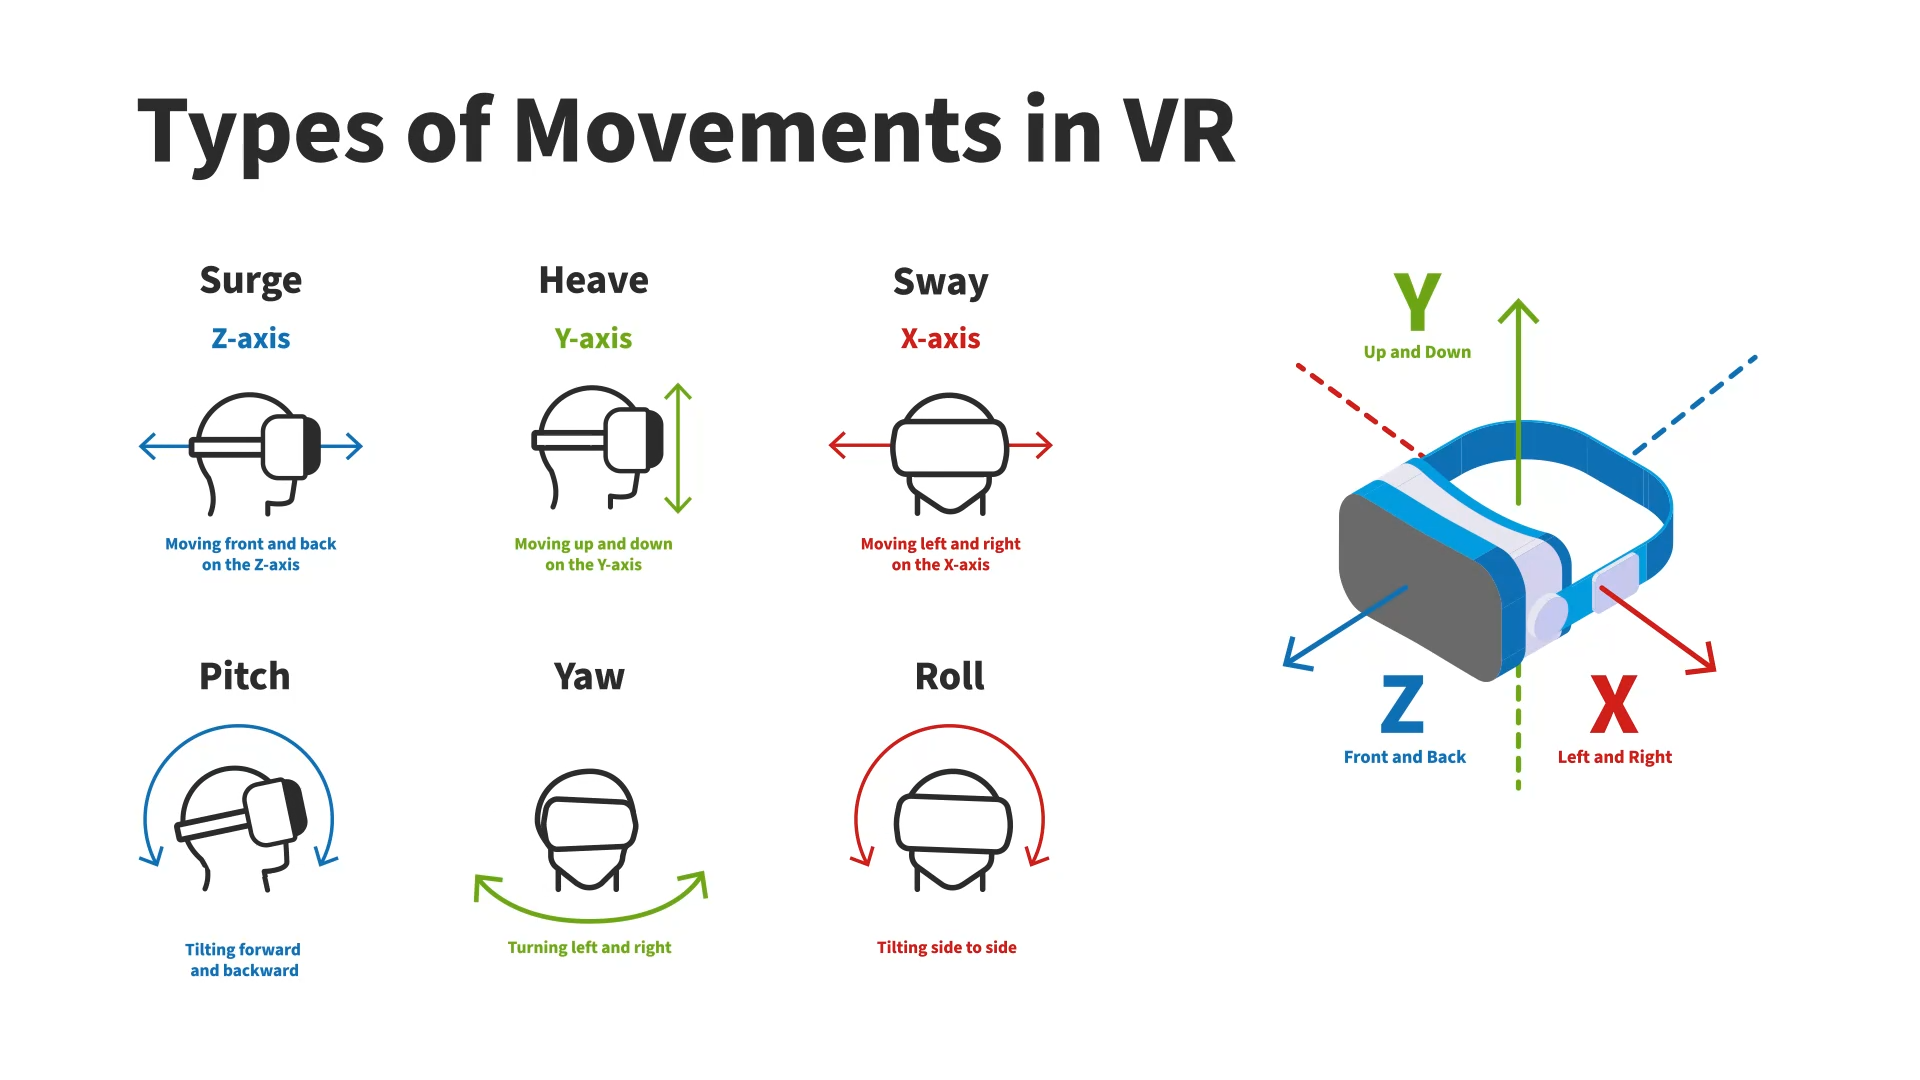
\includegraphics[width=0.85\textwidth]{Ilustración 4.png}
                \label{Ilu4}
            \end{figure}
    \end{frame}

    \begin{frame}
        \frametitle{Panorama actual}
            Según \textbf{International Data Corporation (IDC)}, en 2024, los envíos globales de visores de RA y RV aumentaron un 10\% en comparación con el año anterior, alcanzando aproximadamente 7.5 millones de unidades.\\
            ­\\
            Este crecimiento se atribuye al lanzamiento de nuevos productos y a la entrada de nuevos actores en el mercado.
    \end{frame}

    \begin{frame}
        \frametitle{Panorama actual}
            \begin{figure}
                \centering
                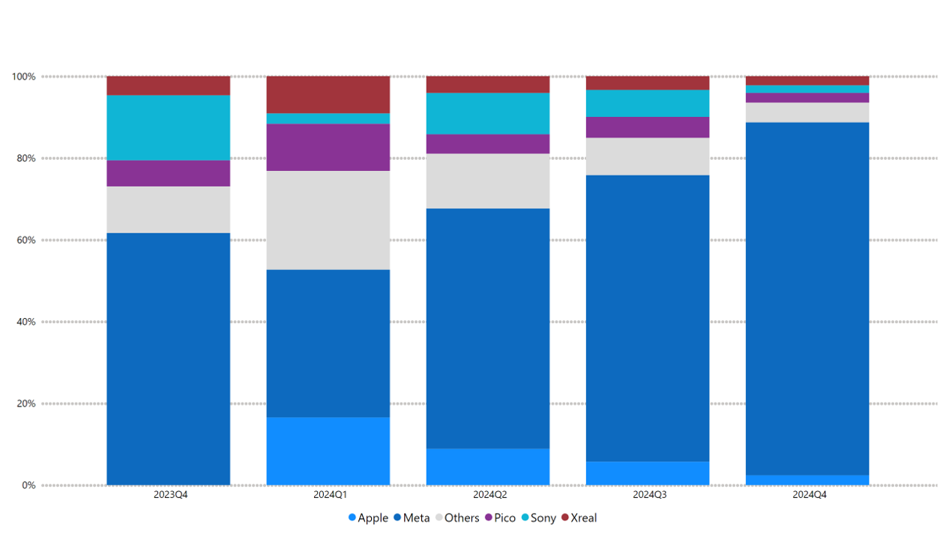
\includegraphics[width=0.8\textwidth]{Gráfica 2.png}
                \label{Gra2}
            \end{figure}
    \end{frame}

    \begin{frame}
        \frametitle{Panorama actual}
            \textbf{Proyecciones para 2025}\\
            \begin{enumerate}
                \item Se anticipa una \textbf{disminución del 12\%} en los envíos de visores AR/VR en 2025.
                \item Se espera un repunte significativo en 2026, con un \textbf{crecimiento del 87\%}. Los envíos superarán los 11.2 millones de unidades.
                \item IDC prevé una \textbf{tasa de crecimiento anual compuesta (CAGR) del 38.6\%} entre 2025 y 2029.
            \end{enumerate}
    \end{frame}    

\section{Entorno de las Meta Quest 3}
    \begin{frame}
        \frametitle{Entorno de las Meta Quest 3}
            \centering
            \textbf{Sección demostrativa.}
    \end{frame}

\section{Futuro de la XR}
    \begin{frame}
        \frametitle{Futuro de la XR}
            \centering
            \textbf{¿Qué podemos esperar para el futuro?}
    \end{frame}

    \begin{frame}
        \frametitle{Futuro de la XR}
            \begin{figure}
                \centering
                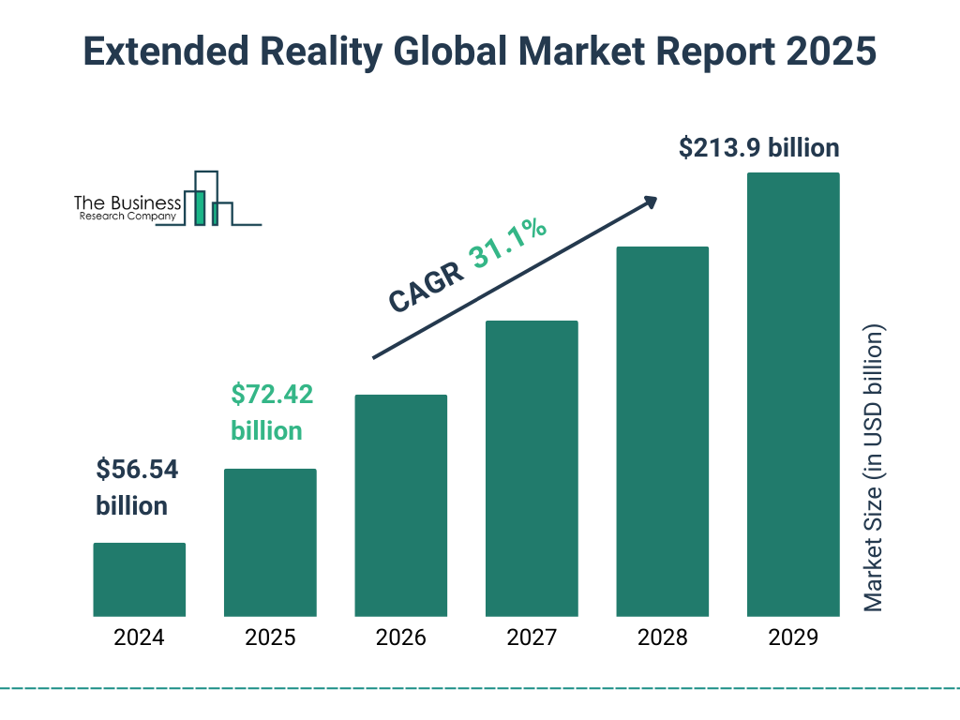
\includegraphics[width=0.65\textwidth]{Gráfica 3.png}
                \label{Gra3}
            \end{figure}
    \end{frame}

    \begin{frame}
        \frametitle{Futuro de la XR}
            \begin{figure}
                \centering
                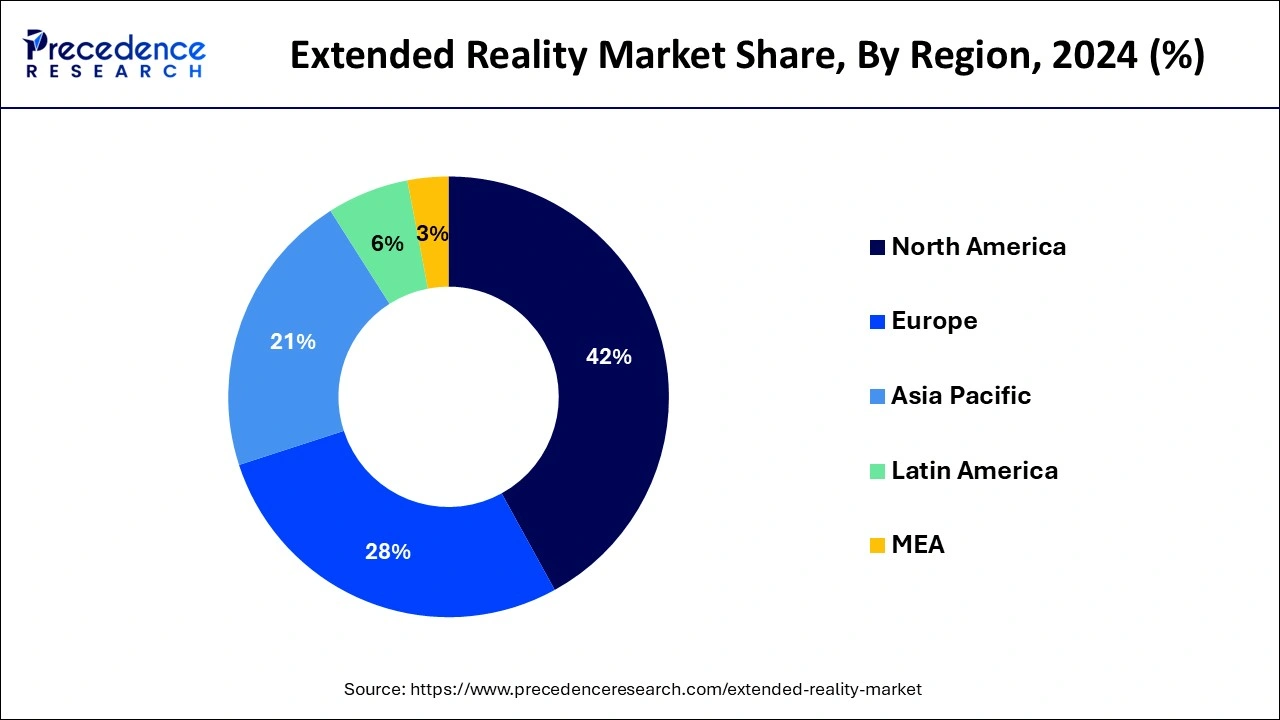
\includegraphics[width=0.8\textwidth]{Gráfica 4.png}
                \label{Gra4}
            \end{figure}
    \end{frame}

    \begin{frame}
        \frametitle{Futuro de la XR}
            \begin{figure}
                \centering
                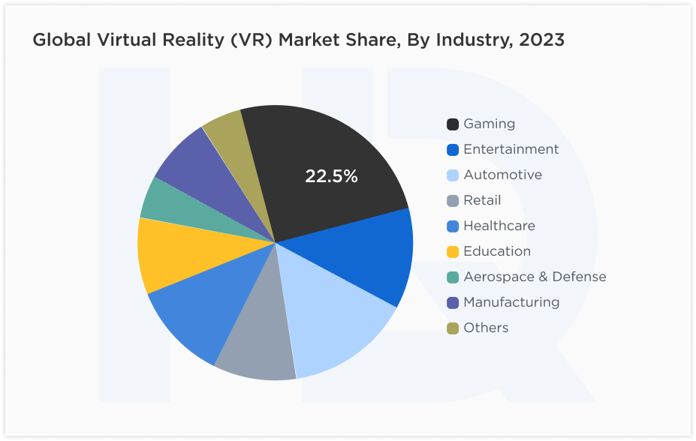
\includegraphics[width=0.7\textwidth]{Gráfica 5.png}
                \label{Gra5}
            \end{figure}
    \end{frame}

    \begin{frame}
        \frametitle{Futuro de la XR}
             \centering
              \textbf{Convergencia de AI + XR}
    \end{frame}
    
    \begin{frame}
        \frametitle{Conclusión}
            \begin{enumerate}
                \item Impacto de la XR en las distintas industrias.
                \item El camino de la IA en el mundo de las XR.
                \item Python, el lenguage del presente.
                \item Importancia de mantenerse en constante actualización.
            \end{enumerate}
    \end{frame}

    \begin{frame}
        \frametitle{Bibliografía}
    \end{frame}
        
\end{document}